% Copyright (c) 2016-2020 The ALF project.
% This is a part of the ALF project documentation.
% The ALF project documentation by the ALF contributors is licensed
% under a Creative Commons Attribution-ShareAlike 4.0 International License.
% For the licensing details of the documentation see license.CCBYSA.

% !TEX root = doc.tex

%-----------------------------------------
%\section{Auxiliary Field Quantum Monte Carlo: projective algorithm}\label{sec:defT0}
%-----------------------------------------

The projective approach is the method of choice if  one is interested in ground-state properties.  The starting point is a pair of trial wave functions,  $| \Psi_{T,L/R} \rangle $, that are  not orthogonal to the ground state $| \Psi_0 \rangle $:
\begin{equation}
  \langle \Psi_{T,L/R}  | \Psi_0 \rangle  \neq 0. 
\end{equation}
The ground-state expectation value of  any  observable  $\hat{O} $ can then be computed by  propagation along the imaginary time axis:
  \begin{equation}
	 \frac{ \langle \Psi_0 | \hat{O} | \Psi_0 \rangle }{ \langle \Psi_0 | \Psi_0 \rangle}   = \lim_{\theta \rightarrow \infty}  
	 \frac{ \langle \Psi_{T,L} | e^{-\theta \hat{H}}  e^{-(\beta - \tau)\hat{H}  }\hat{O} e^{- \tau  \hat{H} }   e^{-\theta \hat{H}} | \Psi_{T,R} \rangle } 
	        { \langle \Psi_{T,L} | e^{-(2 \theta + \beta) \hat{H}  } | \Psi_{T,R} \rangle } ,
\end{equation}
where $\beta$ defines the imaginary time range where observables (time displaced and equal time) are measured and $\tau$ varies from $0$ to $\beta$ in the calculation of time-displace observables.
The simulations are carried out at large  but finite values of  $\theta$ so as to guarantee convergence to the ground  state within the statistical uncertainty.
The trial wave functions are determined up to a phase, and the program uses this gauge choice to  guarantee that
\begin{equation}
	 \langle \Psi_{T,L} | \Psi_{T,R} \rangle  > 0.
\end{equation}
In order to use the projective version of the code, the model's namespace in the \texttt{parameter} file must set \texttt{projector=.true.} and specify the value of the projection parameter \texttt{Theta}, as well as the imaginary time interval \texttt{Beta} in which observables are measured.

Note that time-displaced correlation functions  are computed for a $\tau$ ranging from $0$ to $\beta$.  The implicit assumption  in this formulation is that  the projection  parameter  \texttt{Theta}  suffices to reach the ground state.    Since the  computational time scales linearly with  \texttt{Theta}   large projections parameters are computationally not expensive. 


\subsection{Specification of the trial wave function} \label{sec:trial_wave_function}

For each flavor, one needs to specify a left and a right trial wave function. In the ALF, they are assumed to be the ground state of single-particle trial Hamiltonians $\hat{H}_{T, L/R}$ and hence correspond to a single Slater determinant each. More specifically, we consider a single-particle Hamiltonian with the same symmetries (color and flavor) as the original Hamiltonian:
\begin{equation} \label{eq:trial_wave_function}
\hat{H}_{T,L/R} = 
\sum\limits_{\sigma=1}^{N_{\mathrm{col}}}
\sum\limits_{s=1}^{N_{\mathrm{fl}}}
\sum\limits_{x,y}^{N_{\mathrm{dim}}}
\hat{c}^{\dagger}_{x \sigma   s} h_{xy}^{(s, L/R)} \hat{c}^{\phantom\dagger}_{y \sigma s}.
\end{equation}
Ordering the eigenvalues  of the Hamiltonian in ascending order yields the ground state
\begin{equation}
	 | \Psi_{T,L/R} \rangle    =     \prod_{\sigma=1}^{N_{\mathrm{col}}}  \prod_{s=1}^{N_{\mathrm{fl}}}      \prod_{n=1}^{N_{\mathrm{part},s}} 
	 \left( \sum_{x=1}^{N_{\mathrm{dim}}}    \hat{c}^{\dagger}_{x \sigma   s} U^{(s, L/R)}_{x,n} \right) 
	  | 0 \rangle ,
\end{equation} 
where 
\begin{equation}
	U^{\dagger,(s, L/R)}h^{(s, L/R)}  U^{(s, L/R)}   = \mathrm{Diag} \left(   \epsilon_1^{(s, L/R)}, \cdots, \epsilon_{N_{\mathrm{dim}}}^{(s, L/R)} \right).
\end{equation}
The trial wave function is hence  completely defined by the set of orthogonal vectors  $ U^{(s, L/R)}_{x,n} $  for  $ n $ ranging from  $ 1 $ to  the number of particles   in each flavor sector, $N_{\mathrm{part},s}$.  This information  is stored in the \texttt{WaveFunction}  type defined in the module \texttt{WaveFunction\_mod} (see Sec.~\ref{sec:wave_function}).  Note that, owing to the SU(N$_{\mathrm{col}}$) symmetry, the color index is not necessary to define  the trial wave function.  The user will have to specify the trial wave function in the following way:
\begin{lstlisting}[style=fortran,escapechar=\#]
Do s = 1, N_fl
   Do x = 1,Ndim
      Do n = 1, N_part(s)
         WF_L(s)%P(x,n)  = #  $U${\tiny $^{(s, L)}_{x,n}$}  #
         WF_R(s)%P(x,n)  = #  $U${\tiny $^{(s, R)}_{x,n}$}  #
      Enddo
   Enddo
Enddo
\end{lstlisting}
In the above \texttt{WF\_L} and \texttt{WF\_R} are \texttt{WaveFunction} arrays of length $N_{\mathrm{fl}}$. ALF comes with a set of predefined trial wave functions, see Sec.~\ref{sec:predefined_trial_wave_function}.

Generically,   the  unitary matrix    will  be generated by a
diagonalization routine such that  if the ground state for the given particle number is degenerate, the trial wave function  has a degree of ambiguity  and does not necessarily share the symmetries of the Hamiltonian $\hat{H}_{T, L/R}$.   Since symmetries are the key for guaranteeing the absence of the negative sign problem, violating them in the choice of the trial wave function can very well lead to a  sign problem.   It is hence recommended to define the trial Hamiltonians $\hat{H}_{T, L/R}$ such that the ground state  for the given  particle number is non-degenerate. That can be checked using the value of \texttt{WL\_L/R(s)\%Degen}, which stores the energy difference between the last occupied and first un-occupied single particle state. If this value is greater than zero, then the trial wave function is non-degenerate and hence has all the symmetry properties of the trial Hamiltonians, $\hat{H}_{T, L/R}$. When the \texttt{projector} variable is set to \texttt{.true.}, this quantity is listed in the \texttt{info} file. 

\subsection{Some technical aspects of the projective code.}
If one is interested solely in zero-temperature properties, the projective code offers many advantages.  This comes from the related facts that the Green function matrix is a projector, and that scales can be omitted. 
  
In the projective algorithm, it is known \cite{Assaad08_rev} that 
\begin{equation}\label{eqn:GreenT0_eq}
G(x,\sigma,s,\tau| x',\sigma,s,\tau)  =    \left[ 1 -  U^{>}_{(s)}(\tau)  \left(   U^{<}_{(s)}(\tau) U^{>}_{(s)}(\tau)  \right)^{-1}  U^{<}_{(s)}(\tau) \right]_{x,x'}
\end{equation}
with 
\begin{equation}
  U^{>}_{(s)}(\tau)  =    \prod_{\tau'=1}^{\tau} \bm{B}_{\tau'}^{(s)}   P^{(s),R}  \quad \text{and}  \quad 
  U^{<}_{(s)}(\tau)  =    P^{(s),L, \dagger} \prod_{\tau'=L_{\text{Trotter}} }^{\tau+1} \bm{B}_{\tau'}^{(s)} ,
\end{equation} 
where $\bm{B}_{\tau}^{(s)}$ is given by Eq.~\eqref{Btau.eq} and $P^{(s),L/R}$  correspond to the $N_{\mathrm{dim}} \times N_{\mathrm{part},s} $  submatrices of $U^{(s),L/R}$.   To see that scales can be omitted, we carry out a singular value decomposition: 
\begin{equation}
	U^{>}_{(s)}(\tau)  =\tilde{U}^{>}_{(s)}(\tau)   d^{>} v^{>}   \quad \text{and}  \quad \;  U^{<}_{(s)}(\tau)  = v^{<}  d^{<} \tilde{U}^{<}_{(s)}(\tau)   
\end{equation}
such that $ \tilde{U}^{>}_{(s)}(\tau) $ corresponds to a set of column-wise orthogonal vectors. It can be readily seen that scales can be omitted, since
\begin{equation}
G(x,\sigma,s,\tau| x',\sigma,s,\tau)  =    \left[ 1 -  \tilde{U}^{>}_{(s)}(\tau)  \left(   \tilde{U}^{<}_{(s)}(\tau) \tilde{U}^{>}_{(s)}(\tau)  \right)^{-1}  \tilde{U}^{<}_{(s)}(\tau) \right]_{x,x'}.
\end{equation}
Hence, stabilization is never an issue for the projective code, and arbitrarily large projection parameters  can be reached.  
 
The form of the Green function matrix implies that it is a projector: $G^2 = G$.   This property has been used in Ref.~\cite{Feldbach00} to very efficiently compute imaginary-time-displaced correlation functions.  



\subsection{Comparison of finite and projective codes.}
\label{Sec:Compare_T0_T}
The finite temperature code  operates in the grand canonical ensemble, whereas  in the projective   approach  the particle number is fixed.  On finite lattices, the comparison between both approaches can only  be made at a temperature scale below which a finite-sized charge gap  emerges.  In Fig.~\ref{PQMC.fig}  we consider a semi-metallic phase  as realized by    the Hubbard model on the Honeycomb lattice  at $U/t=2$. It is evident that, at a scale below which charge fluctuations are  suppressed, both algorithms yield identical results. 
        
\begin{figure}
\center
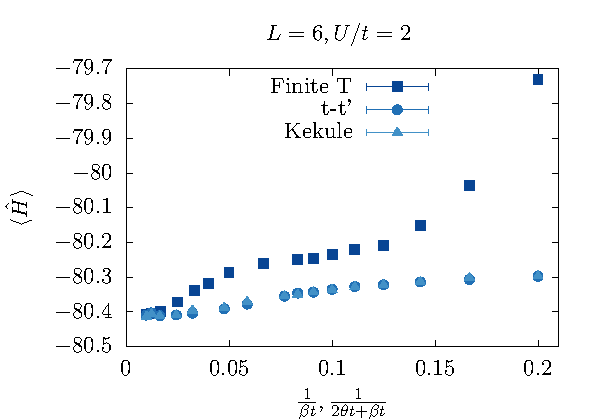
\includegraphics[width=0.49\textwidth]{Figures/Projector/Proj_ener.pdf}
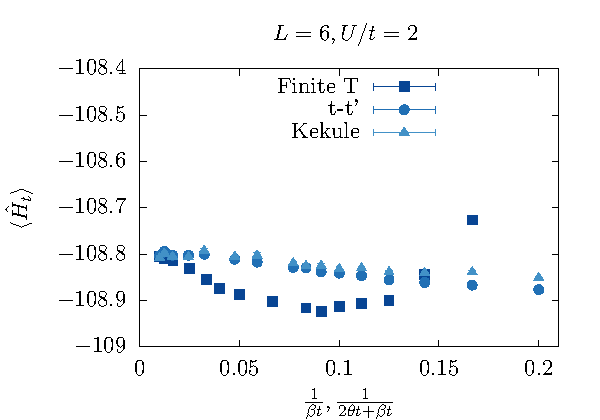
\includegraphics[width=0.49\textwidth]{Figures/Projector/Proj_kin.pdf} \\
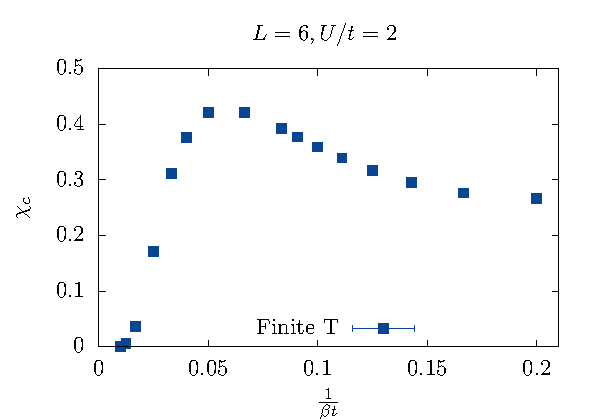
\includegraphics[width=0.49\textwidth]{Figures/Projector/Proj_chi.pdf}

	\caption{Comparison between the finite-temperature and projective codes for the Hubbard model on a $6 \times 6 $  Honeycomb lattice at $U/t=2$ and with periodic boundary conditions.   For the projective code (blue and black symbols) $\beta t = 1$ is fixed, while $\theta$ is varied. In all cases we have $\Delta \tau t = 0.1$, no checkerboard decomposition, and a symmetric Trotter decomposition.  For this lattice size and choice of boundary conditions, the non-interacting ground state is degenerate, since the Dirac points belong to the discrete set of crystal momenta.  In order to generate the trial wave function we  have lifted this degeneracy by either including a K\'ekul\'e mass term \cite{Lang13} that breaks translation symmetry (blue symbols), or by adding a next-next nearest neighbor hopping (black symbols) that breaks the symmetry nematically and shifts the Dirac points away from the zone boundary~\cite{Ixert14}. As apparent, both choices of trial wave functions yield the same answer, which compares very well with the finite temperature code at temperature scales below the finite-size charge gap.}
	\label{PQMC.fig}
\end{figure}

